\documentclass[a4paper,12pt]{report}
\usepackage[utf8x]{inputenc}
\usepackage[brazil]{babel}
\usepackage[T1]{fontenc}
\usepackage{epstopdf}
%\DeclareGraphicsRule{.tif}{png}{.png}{`convert #1 `dirname #1`/`basename #1 .tif`.png}
\usepackage{tikz}
\usepackage{indentfirst}
\hyphenation{li-vro tes-te cha-ve bi-blio-te-ca}
\hyphenation{co-men-t-rio re-fe-rn-cia}
\usetikzlibrary{positioning,shapes,shadows,arrows}
\newcommand{\HRule}{\rule{\linewidth}{0.5mm}}

\linespread{1.5}
\pagestyle{plain}


\begin{document}

%%%%%%%%%%%%%%%%%%%
% parte frontal
%%%%%%%%%%%%%%%%%%%

\begin{titlepage}

\begin{center}


\includegraphics[width=0.15\textwidth]{./logo.jpeg}\\[1cm]

\textsc{\LARGE Universidade Federal do Rio de Janeiro}\\[1.5cm]


% Title
\HRule \\[0.4cm]
{ \huge \bfseries Avaliação e Desempenho }\\[0.4cm]
{ \huge \bfseries Simulador} \\[0.4cm]
\HRule \\[1.5cm]


% Author and supervisor
\begin{minipage}{0.6\textwidth}
  \begin{flushleft} 
  \emph{Componentes:}\\
  Bruno Lima Cardoso \\
  Daniel Santos Ferreira Alves \\
  Mariam dos Passos Afonso da Conceição \\
  Peter Peret Lupo
  \end{flushleft}
\end{minipage}
\begin{minipage}{0.3\textwidth}
  \begin{flushright}
  \emph{DRE:} \\
  108055733 \\
  107362161 \\
  104034913 \\
  101137720
  \end{flushright}
\end{minipage}

\vfill

\begin{minipage}{1.0\textwidth}
  \small Bruno, Daniel e Mariam participaram ativamente, de forma remota ou presencial, de todas as etapas da elaboração do trabalho: definição do funcionamento do simulador, implementação do código, testes e produção do relatório. Peter participou das discussões, auxiliando na definição da infraestrutura do simulador e em revisões de código, fórmulas e bugs.\\
\end{minipage}

\vfill


% Bottom of the page
{\large \today}

\end{center}

\end{titlepage}

\begin{abstract}
\end{abstract}

\chapter*{Siglas}
\begin{list}{$\bullet$}{}
  \item[VA] - Variável Aleatória
  \item[IC] - Intervalo de Confiança
\end{list}

\chapter*{Lista de Variáveis}
\begin{list}{$\bullet$}{}
  \item[$N_{q1}$] - Número de pessoas em espera na fila 1.
  \item[$N_{q2}$] - Número de pessoas em espera na fila 2.
  \item[$N_1$] - Número de pessoas na fila 1.
  \item[$N_2$] - Número de pessoas na fila 2.
  \item[$W_1$] - Tempo de espera da fila 1.
  \item[$W_2$] - Tempo de espera da fila 2.
  \item[$X_1$] - Tempo do primeiro serviço.
  \item[$X_2$] - Tempo do segundo serviço.
  \item[$T_1$] - Tempo total de execução da fila 1.
  \item[$T_2$] - Tempo total de execução da fila 2.
  \item[$\rho$] - Utilização.
\end{list}

\tableofcontents

\listoffigures

\listoftables

%%%%%%%%%%%%%
% Introdução
%%%%%%%%%%%%%
\chapter{Introdução}

\section{Funcionamento Geral do Simulador}
O fluxo de execução do simulador é descrito, a seguir, em linhas gerais.
\begin{itemize}
  \item As estruturas internas são inicializadas e o evento inicial é gerado.
  \item Aguarda-se a execução da fase transiente.
  \item O loop principal de rodadas é iniciado. Para cada rodada:
  \begin{itemize}
    \item Se o critério de parada for satistfeito (todos os ICs são suficientemente pequenos), pare.
    \item A coleta de amostras da rodada é reiniciada.
    \item “n = eventos por rodada” eventos são retirados da fila de eventos e processados.
    \item Se não for a fase transiente, as médias da rodada são calculadas e adicionadas às listas de médias globais.
\end{itemize}
  \item Os resultados encontrados são impressos no terminal.
\end{itemize}

A execução de cada evento é descrita com detalhes na seção que trata dos tipos de eventos.

Mais detalhes sobre o funcionamento do simulador estão no workflow do Anexo %número do anexo

\section{Eventos Escolhidos}
Os eventos utilizados são as chegadas nas filas, e cada fila possui um evento de chegada correspondente.

\section{Estruturas Internas Utilizadas}
Nosso código utiliza as estruturas a seguir.
\begin{itemize}
  \item Um objeto para representa a próxima chegada na primeira fila.
  \item Uma lista para armazenar as chegadas ainda não foram servidas na segunda fila.
\end{itemize}

Não houve necessidade de usarmos uma fila de prioridades, pois os eventos já são inseridos ordenados por tempo.

Também vale destacar que temos mais de uma classe para armazenas as estatísticas coletadas:
\begin{itemize}
  \item \textit{Metrics} - coleta das estatísticas por tipo;
  \item \textit{MetricsCollection} - reúne as estatísticas de xxx por rodada;
  \item \textit{MetricsAgregator} - agrega os valores obtidos por cada rodada.
\end{itemize}

\section{Geração das Variáveis Aleatórias (VA)}
O Java possui classes prontas para fornecer números aleatórios, dentre as quais utilizamos \textit{Random} para obter números pseudo-aleatórios, entre 0 e 1, do tipo \textit{double}. Já a geração de VAs Exponenciais teve de ser implementada, papel da classe \textit{RandomExponentialVariable}. O cálculo do IC exigiu apenas um valor fixo da distribuição t-Student: o percentil \textit{$t_{0,975}$ = 1, 960}. Este valor foi armazenado na variável \textit{t}, da classe \textit{Metrics}. Outras distribuições não foram necessárias.

O método escolhido para geração das rodadas foi o \textit{Batch}, principalmente por ser necessária a realização de somente uma fase transiente, colaborando para a diminuição do tempo execução do simulador. A semente foi escolhida aleatoriamente e mantida ao longo de cada cenário.

\section{Linguagem}
A linguagem escolhida foi \textit{Java 1.6}, devido à sua portabilidade e facilidade de uso. Os gráficos foram desenhados com a ferramente \textit{GNUPlot}. Ambos estão disponíveis para Linux e Windows.

\section{Escolha de Parâmetros}
O tamanho da fase transiente foi determinado empiricamente, testando-se diversos valores. Uma fase transiente inadequada era indicada pela ocorrência de ICs crescentes ao longo da simulação. Desta forma, aumentamos gradualmente o valor de seu tamanho até que os resultados fossem satisfatórios.

As tabelas com os resultados pertinentes estão ...%%%%%.

\section{Especificação da Máquina}
O computador usado para os testes documentados tem sistema operacional Arch Linux, processador Intel i5 e 4GB de memória RAM. Fizemos, também, um breve teste num PC com Windows XP, apenas para certificar que o simulador também era executável nesta plataforma.

\section{Informações Adicionais}
Para rodar o simulador em ambiente linux, basta digitar a seguinte linha de comando:
java -jar simulador.jar

Os parâmetros de simulação podem ser alterados no próprio código, na classe \textit{TextControl}.

%%%%%%%%%%%%%
% Testes
%%%%%%%%%%%%%
\chapter{Testes de Correção}


%%%%%%%%%%%%%
% Fase transiente
%%%%%%%%%%%%%
\chapter{Estimação da Fase Transiente}

\section{Método de Estimação}

\section{Resultados do Processo}

%%%%%%%%%%%%%
% Análise
%%%%%%%%%%%%%
%tabelas com resultados e comentários pertinentes
\chapter{Análise e Desempenho}


%Mude o caminho e descomente
%``graphs/graph-2.png é o caminho relativo da figura a partir do .tex
\begin{figure}[htbp]
   \centering
   \fbox{
	   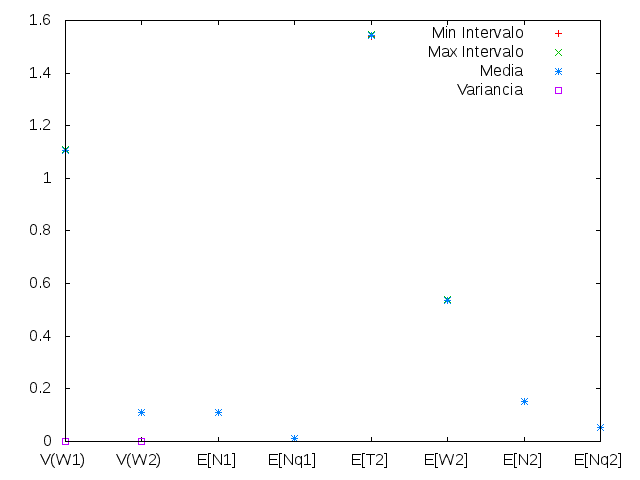
\includegraphics[width=1\textwidth]{graficos/graph-2.png}
   }\caption{Exemplo de uma figura}
\end{figure}

\begin{figure}[htbp]
   \centering
   \fbox{
	   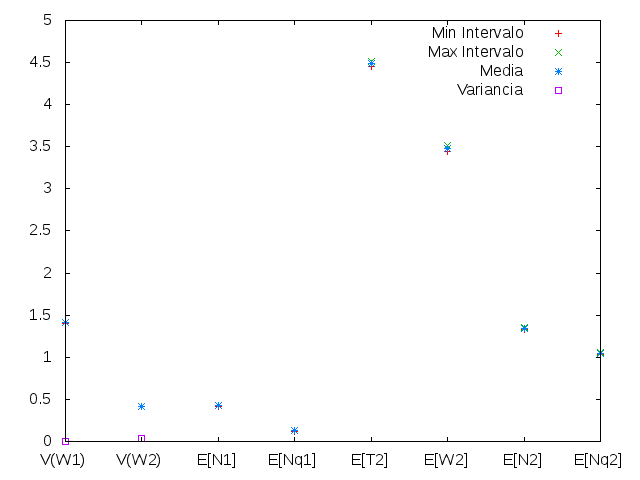
\includegraphics[width=1\textwidth]{graficos/graph-6.png}
   }\caption{Exemplo de uma figura}
\end{figure}

\begin{figure}[htbp]
   \centering
   \fbox{
	   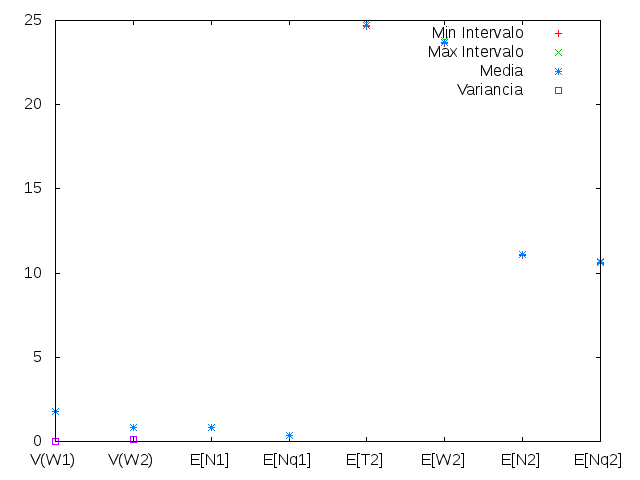
\includegraphics[width=1\textwidth]{graficos/graph-9.png}
   }\caption{Exemplo de uma figura}
\end{figure}

\begin{figure}[htbp]
   \centering
   \fbox{
	   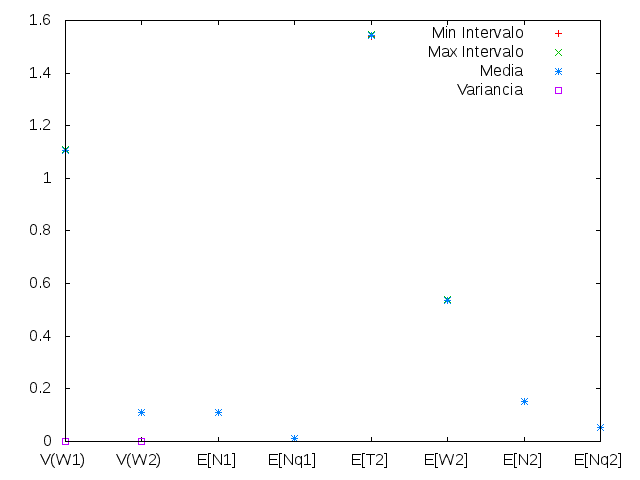
\includegraphics[width=1\textwidth]{graficos/graph-2.png}
   }\caption{Exemplo de uma figura}
\end{figure}

\begin{figure}[htbp]
   \centering
   \fbox{
	   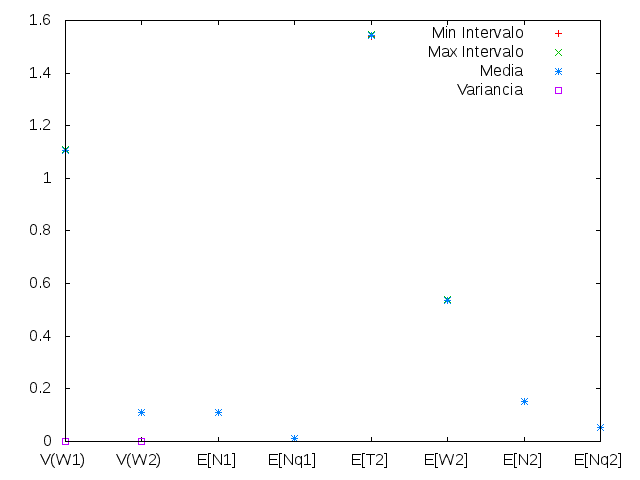
\includegraphics[width=1\textwidth]{graficos/graph-2.png}
   }\caption{Exemplo de uma figura}
\end{figure}

\textbf{Exemplo de tabela}

% uma letra c para cada coluna
% as | representam as barras verticais da tabela
% \hline representa linha horisntal
% & fica entre dados de colunas - se a celela for vazia vc ainda precisa por todos & - exemplo a23 e a32

\[
  \begin{array}{|c|c|c|}
    \hline
    cel1 & cel2 & cel3 \\ \hline
    cel1 & cel2 &      \\ \hline
         & cel2 & cel3 \\ \hline
  \end{array}
\]



%%%%%%%%%%%%%
% Otimização
%%%%%%%%%%%%%
\chapter{Otimização}

\section{Apresentação do Método}

\section{Análise Gráfica de Resultados}

%%%%%%%%%%%%%
% Conclusão
%%%%%%%%%%%%%
\chapter{Conclusão}


%%%%%%%%%%%%%%%%%%%
% parte final
%%%%%%%%%%%%%%%%%%%

\appendix
\chapter{O Programa}

\newpage

\section{Workflow}

\tikzstyle{decision} = [diamond, draw, fill=green!20, text width=4em, text badly centered, node distance=4cm, inner sep=0pt]
\tikzstyle{block} = [rectangle, draw, fill=blue!20, text width=5em, text centered, rounded corners, minimum height=4em]
\tikzstyle{line} = [draw, -latex']
\tikzstyle{cloud} = [draw, ellipse,fill=red!20, node distance=5cm, minimum height=2em]
\tikzstyle{start} = [draw, circle, fill=black, node distance5em, minimum height=1em]
    
\begin{tikzpicture}[node distance = 3cm, auto]
    % Place nodes
    \node [cloud] (init) {início};
    \node [block, right of=init] (seed) {seleciona semente};
    \node [block, right of=seed] (processtrans) {fase transiente};
    \node [block, below of=processtrans] (processrod) {processa m eventos};
    \node [block, left of=processrod] (colectdata) {coleta estatisticas};
    \node [decision, below of=colectdata] (decideic) {tamanho mínimo de IC?};
	\node [block, left of=decideic, node distance=5cm] (processextra) {processa outro evento};
    \node [block, below of=decideic, node distance=4cm] (groupdata) {agrupa os dados das rodadas};
	\node [decision, below of=groupdata] (minrodadas) {nº mim de rodadas?};
    \node [block, below of=minrodadas] (estatgeral) {obtem estatísticas gerais};
    \node [decision, right of=estatgeral, node distance=4.5cm] (decideicgeral) {achou IC?};
    \node [cloud, right of=decideicgeral, node distance=3cm] (stop) {fim};
    % Draw edges
    \path [line] (init) -- (seed);
    \path [line] (seed) -- (processtrans);
    \path [line] (processtrans) -- (processrod);
    \path [line] (processrod) -- (colectdata);
    \path [line] (colectdata) -- (decideic);
    \path [line] (decideic) -- node {não} (processextra);
    \path [line] (decideic) -- node {sim} (groupdata);
	\path [line] (processextra) |- (colectdata);
    \path [line] (groupdata) -- (minrodadas);
	\path [line] (minrodadas) -| node {não} (processrod);
	\path [line] (minrodadas) -- node {sim} (estatgeral);
    \path [line] (estatgeral) -- (decideicgeral);
    \path [line] (decideicgeral) |- node {não} (processrod);
    \path [line] (decideicgeral) -- node {sim} (stop);
\end{tikzpicture}

\end{document}          
